\documentclass{beamer}


\usepackage[english]{babel}
\usepackage[latin1]{inputenc}
\usepackage{times}
\usepackage[T1]{fontenc}
\usepackage{amsbsy}         % for \boldsymbol command (bold in math mode)
\usepackage{amsfonts, amssymb}
\usepackage{epsfig}
\usepackage{color}
\definecolor{camblue}{RGB}{26,26,89}
\definecolor{Rblue}{RGB}{0,255,255}
\definecolor{Rdarkblue}{RGB}{0,0,255}
\definecolor{Rgreen}{RGB}{0,205,0}
\newcommand{\tcb}{\textcolor{beamer@blendedblue}}
\newcommand{\tcbb}{\textcolor{camblue}}
\newcommand{\tcr}{\textcolor{red}}
\newcommand{\tcg}{\textcolor{gray}}
\newcommand{\tcRg}{\textcolor{Rgreen}}
\newcommand{\tcRdb}{\textcolor{Rdarkblue}}
\newcommand{\tcRb}{\textcolor{Rblue}}
\newcommand{\sq}{\begin{eqnarray}}
	\newcommand{\fq}{\end{eqnarray}}
\newcommand{\bp}{$\bullet$\:}
\begin{document}

%------------------------------------------------------------------------%
\section[Intro to MCS]{Introduction to Method Comparison Studies}
\subsection{Method Comparison Studies}
\begin{frame}{\bf \tcb{Bland-Altman Plot}}
	\vspace{-0.9cm}
	\begin{itemize}\itemsep0.5cm
		\item Method Comparison: Commonly encountered issue in medical statistics
		\item ``Do two methods of measurement agree statistically?".
		\item ``Can the two methods be used interchangeably?"
		\item Sources of disagreement can arise from differing population means (i.e. inter-method bias), differing between-subject and with-in subject variances \textit{(Anuradha Roy 2009)}.
	\end{itemize}
	
\end{frame}
%------------------------------------------------------------------------%

\begin{frame}{\bf \tcb{The Bland-Altman Plot}}
	\vspace{-1cm}
	\begin{itemize}\itemsep0.5cm
		
		\item The Bland-Altman plot is a very simple graphical method to compare two measurements techniques. \item In this approach the case-wise differences between the two methods are plotted against the corresponding case-wise averages of the two methods.
		
		\item A horizontal lines is drawn at the mean difference(the inter-method bias) , and at the limits of agreement, which are defined as the inter-method bias plus and minus 2 times the standard deviation of the differences.
		
	\end{itemize}
\end{frame}

\begin{frame}[fragile]
	\frametitle{Bland-Altman Plot}
	\vspace{-1cm}
	\begin{verbatim}
	>X = rnorm(14,6,1);Y = rnorm(14,5.3,1.1)
	>
	>A=(X+Y)/2		#case-wise averages
	>D=X-Y			#case-wise differences
	>		
	>Dbar=mean(D)	#inter-method bias
	>SdD=sd(D)		#standard deviation of the differences
	>
	>plot(A,D,pch=16,col="red", ylim=c(-3,3))
	>
	>abline(h=Dbar,lty=2)
	>abline(h=(Dbar-2*SdD),lty=2)
	>abline(h=(Dbar+2*SdD),lty=2)
	\end{verbatim}
\end{frame}


\begin{frame}
	\frametitle{Simple Bland-Altman Plot}
	
	Inter-method Bias : 0.45 \\
	Limits of Agreement: [-1.32, 2.23]
	\begin{center}
		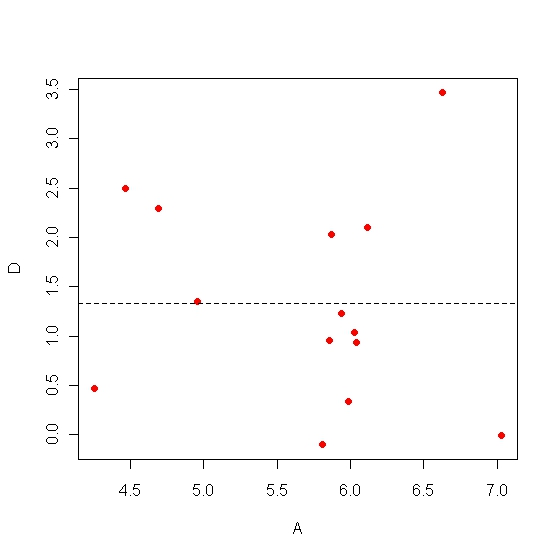
\includegraphics[scale = 0.40]{SimpleBAplot}
	\end{center}
\end{frame}



%------------------------------------------------------------------------%

\begin{frame}{\bf \tcb{The Bland-Altman Plot: Prevalence}}
	\begin{itemize}\itemsep0.7cm
		
		\item Limits of Agreement are used extensively in medical literature for assessing agreement between two methods.
		\item According to Google Scholar, Bland and Altman's 1986 paper has 22,456 citations. \\(``The Pricing of Options and Corporate Liabilities" by Black and Scholes has 19,019 citations.)
	\end{itemize}
\end{frame}

%------------------------------------------------------------------------%

\end{document}
